\documentclass[11pt,a4paper]{article}
\usepackage[utf8]{inputenc}
\usepackage[margin=2cm]{geometry}
\usepackage{graphicx}
\usepackage{booktabs}
\usepackage{tabularx}
\usepackage{url}
\setlength{\parindent}{0pt}
\setlength{\parskip}{4pt}

\begin{document}

\begin{center}
{\large\bfseries Informe del aporte práctico: TurnoJusto}\\[2pt]
Apunte Pazmiño Washington German --- Aplicaciones Distribuidas (ISR-701)
\end{center}

\section*{1. Escenarios ejecutados}
\renewcommand{\arraystretch}{1.15}
\begin{tabularx}{\textwidth}{@{}l c X@{}}
\toprule
\textbf{Esc.} & \textbf{Captura} & \textbf{Interpretación de lo observado}\\
\midrule

E0 & 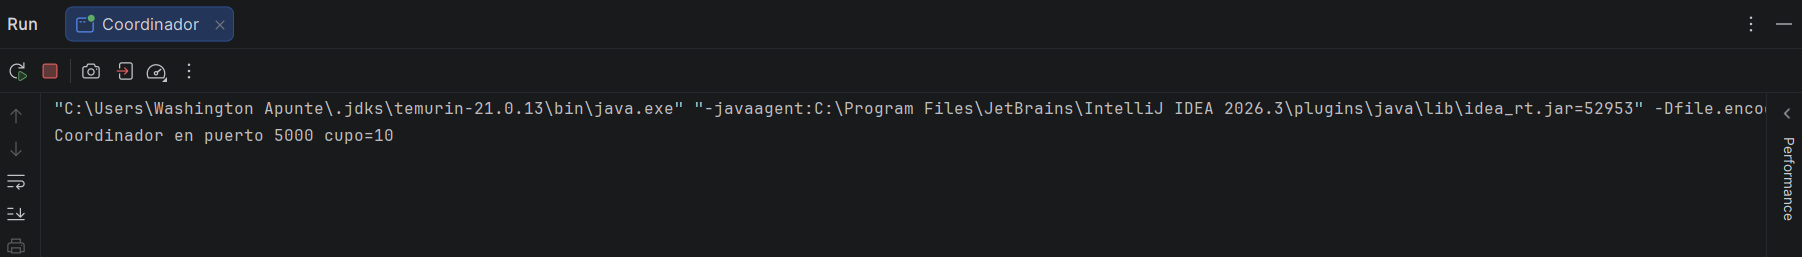
\includegraphics[width=4.2cm]{img/Corrdinadorpuerto5000cupo10.png} & Corrdinador en puerto 5000 y cupo igual a 10.\\
E1 & 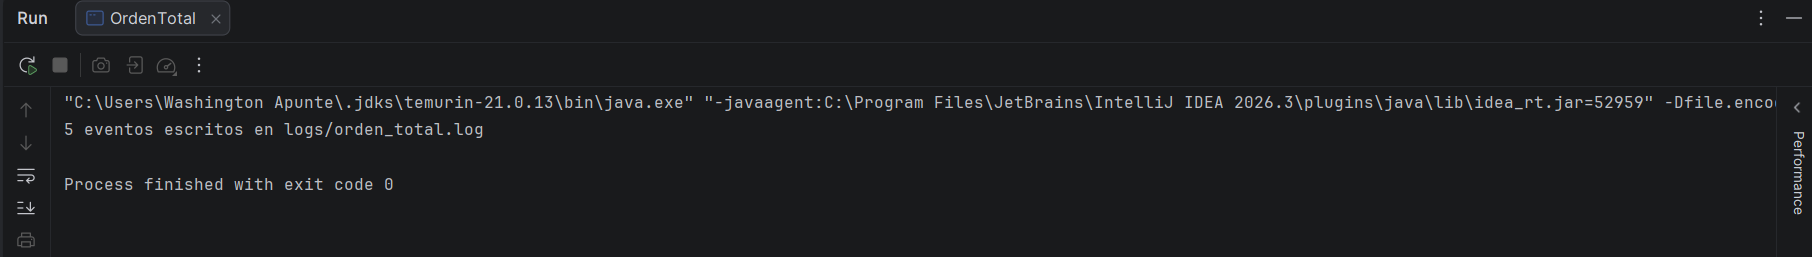
\includegraphics[width=4.2cm]{img/eventosescritosordentotal.png} & Eventos inscritos 5 en log, ordenTotal.\\
E2 & 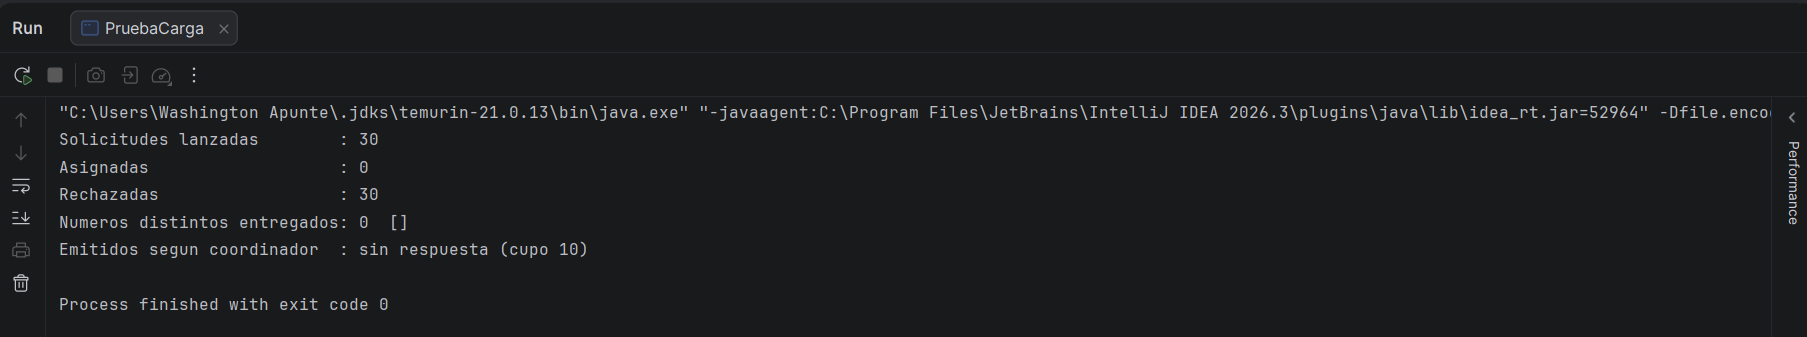
\includegraphics[width=4.2cm]{img/pruebaCarga.png} & Prueba con carga de datos.\\

\bottomrule
\end{tabularx}


\section*{2. Cifras de E3}
\begin{tabular}{@{}lcccc@{}}
\toprule
\textbf{Modo} & \textbf{Asignadas} & \textbf{Rechazadas} & \textbf{Números distintos} & \textbf{Emitidos (coord.)}\\
\midrule
Normal & 30 & 0 & 30 & 20\\

\bottomrule
\end{tabular}

\section*{3. Pares causales de E6}
Par 1: (Asigna 10 cupos\texttt{orden\_total.log}) \ldots\\


\section*{4. Preguntas de análisis}
\textbf{1. Porque rechaza los los logs.} \ldots\\





\end{document}
